\documentclass{article}
\usepackage{amsmath, amsfonts, amsthm, amssymb, wasysym, txfonts, mathrsfs, fancyhdr, multicol, graphicx}


\usepackage[margin=1in]{geometry}

\usepackage{tikz}
\usetikzlibrary{positioning,chains,fit,shapes,calc,arrows,patterns}
\usepackage{xcolor}
\usepackage{colortbl}

\newtheorem{thm}{Theorem}[section]
\newtheorem{co}[thm]{Corollary}
\newtheorem{lem}[thm]{Lemma}
\newtheorem{conj}[thm]{Conjecture}
\newtheorem{assumption}[thm]{Assumption}
\newenvironment{assum}{\begin{assumption}\rm}{\end{assumption}}
\newtheorem{pr}[thm]{Proposition}
\newtheorem{crit}[thm]{Criterion}
\newtheorem{prob}[thm]{Problem}
\newtheorem{definition}[thm]{Definition}
\newenvironment{defi}{\begin{definition}\rm}{\end{definition}}
\newtheorem{example}[thm]{Example}
\newenvironment{exa}{\begin{example}\rm}{\end{example}}
\newtheorem{remark}[thm]{Remark}
\newenvironment{rem}{\begin{remark}\rm}{\end{remark}}


\newcommand{\gretchen}[1]{{\color{blue} \sf Gretchen: #1}}
\newcommand{\emily}[1]{{\color{teal} \sf Emily: #1}}
\newcommand{\andrea}[1]{{\color{gray} \sf Andrea: #1}}
\newcommand{\collin}[1]{{\color{red} \sf Collin: #1}}
\newcommand{\julian}[1]{{\color{violet} \sf Julian: #1}}
\newcommand{\liz}[1]{{\color{olive} \sf Liz: #1}}
\newcommand{\name}[1]{{\color{purple} \sf Name: #1}}
\newcommand{\renaya}[1]{{\color{orange} \sf Renaya: #1}}

\title{Project 2 - McMillon}


\begin{document}

\maketitle

\section*{08/30/23}

\section*{09/06/23}
\subsection{Gallager A/B}

\begin{enumerate}
    \item Only flip Variable Node (VN) if all neighboring Check Nodes (CN) are unsatisfied.
    \item Flip when at least half of the neighboring check nodes are unsatisfied.
    \item Flip when any CN neighbor is unsatisfied.
\end{enumerate}

\section*{9/13/23}

Names for writing things!
\begin{enumerate}
    \item \gretchen{We have colors!}
    \item \emily{Use them!}
    \item \andrea{This way we can tell who has written what in the document.}
    \item \collin{The colors are ok?}
    \item \julian{Latex has a limited number of predefined colors.}
    \item \liz{So we do our best.}
    \item \name{With what we have...}
    \item \renaya{Hopefully this works well!}
\end{enumerate}

\emily{Agenda:
    \begin{enumerate}
        \item Ask about reading.
        \item Define absorbing sets rigorously, draw some, explain why decoding fails.
        \item Activity: work on if the threshold is different, i.e., if the number of unsatisfied check nodes required to flip is at least 1. Try to explore/make conjectures using graphs with 3-4 variable nodes.
    \end{enumerate}}

\section*{9/27/23}

In our standard definition of absorbing set, if a check node has degree $\text{deg}(v) = u + s$ where $s$ is the number of satisfied check nodes and $u$ is the number of unsatisfied check nodes, our decoder rule is that we change the value of $v$ if $u \geq s$. What happens if we change the decoder rule so that:
\begin{itemize}
    \item We change the value of $v$ if $u \geq s + 1$.
    \item We change the value of $v$ if $u \geq s - 1$.
\end{itemize}
The answer should be a characterization of types of graphs, similar to the characterization of absorbing sets, where the number of odd degree neighbors of any variable node was strictly less than the number of even degree variable nodes. It might be good to start with some conventional absorbing sets and alter them.

\section{9/28/23}


\section*{10/4/2023}

When is a standard absorbing set still an absorbing set? What if our update rule is $u \geq s + 1$ or $u \geq s - 1$?

\section*{10/11/2023}

Prove that absorbing sets with the $u \geq s$ update rule are still absorbing sets with the $u \geq s + 1$ update rule.

\begin{definition}
    A $(a \mid b)$ absorbing set is a set of variable nodes that, under the $a \geq b$ update rule, the set of variable nodes is not eventually correct.
\end{definition}


\begin{thm}
    All $(u\mid s)$-absorbing sets are $(u\mid s+1)$-absorbing sets.
\end{thm}



% \begin{proof}

%     Assume that $(u \mid s)$ is an arbitrary absorbing set. Then, for all $v \in S$, the inequality $D_e(v) > D_o(v)$ holds. Initializing all variable nodes with $1$, we have $s = D_e(v)$ and $u = D_o(v)$. As $u < s < s + 1$ we get the inequality $u \geq s + 1$ is never satisfied.
% \end{proof}



\begin{proof}
    Let $V$ denote the set of variable nodes. Assume $(u\mid s)$ is an arbitrary absorbing set, meaning for all $v\in V$, $D_e(v)>D_o(v)$ holds. Initializing all variable nodes with $1$, we have $D_e(v)+1>D_o(v)$ for all $v\in V$. Therefore, $u\geq s+1$ is never satisfied, implying that $(u\mid s)$ is also a $(u\mid s+1)$-absorbing set.
\end{proof}
    
    


\begin{thm}
    All $(u\mid s)$-absorbing sets are $(u\mid s+k)$-absorbing sets.
\end{thm}

\begin{conj}
    Not all $(u\mid s)$-absorbing sets are $(u\mid s-1)$-absorbing sets.
\end{conj}

Gretchen's challenge: Can you come up with things that are $(u \mid s + 1)$-absorbing sets but not $(u \mid s)$-absorbing sets?

If $(u \mid s)$ implies $(u \mid s + k)$, does that mean that $(u \mid s - k)$ implies $(u \mid s)$?


\begin{co}
    If $(u\mid s)$ is an absorbing set then $(u\mid s+k)$ is an absorbing set where $k\in \mathbb{N}_0$
\end{co}

\begin{proof}
Assume that $(u\mid s)$ is an absorbing set and that there exists some $k \in \mathbb{N}$ such that $(u\mid s+k)$ is not an absorbing set. Then, by the well-ordering principle, there exists the smallest $k \in \mathbb{N}$ such that $(u\mid s+k)$ is not an absorbing set. As $(u\mid s+k)$ is the smallest $k$ that is not an absorbing set, then $(u\mid s+k-1)$ is an absorbing set. By Theorem 1.2, $(u\mid s+k)$ is also an absorbing set, a contradiction. Therefore, $(u\mid s+k)$ is an absorbing set.
\end{proof}

\begin{proof}
    Assume that $(u\mid s)$ is an absorbing set. Then set $k=0$ as therefore $(u\mid s+0)$ is also an absorbing set. Now assume that $\exists k \in \mathbb{N}$ s.t. $(u \mid s +k)$ is an absorbing set. Then by Theorem 1.2 $(u\mid s+k+1)$ is also an absorbing set.
\end{proof}

\section*{10/25/2023}


\begin{thm}
    If every $v \in S$ is such that $v$ has \textit{exactly} $t$ more even degree than odd degree neighbors in $G_S$, then $S$ is not an $(u \mid s - t)$ absorbing set. It is a $(u \mid s - k)$ absorbing set for all $k < t$.
\end{thm}
\begin{proof}

    Assuming that for all $v \in S$, the equality $D_e(v) = D_o(v) + t$ holds, where $t \in \mathbb{N}_0$. If every variable node is initialized with $1$, then $D_e(v) = s$ and $D_o(v) = u$. Under the update rule $u \geq s - t$, this would not be an absorbing set, as $D_o(v) = D_e(v) - t$ would cause every variable node to switch on the first iteration of the algorithm.

    Under the update rule $u\geq s-k$ where $k<t$, this would be an absorbing set as $u\geq u+t-k$ would never be satisfied.
\end{proof}


\begin{thm}
    If every $v \in S$ is such that $v$ has at least $t$ more even degree than odd degree neighbors in $G_S$, then $S$ is a $(u \mid s - t + 1)$ absorbing set.
\end{thm}
\begin{proof}
    Assuming that for all $v \in S$, the inequality $D_e(v) \geq D_o(v) + t$ holds, where $t \in \mathbb{N}_0$. If every variable node is initialized with $1$, then $D_e(v) = s$ and $D_o(v) = u$. Under the update rule $u \geq s - t + 1$, this would not be an absorbing set, as $s + 1 \leq u + t \leq s$ is never satisfied.
\end{proof}

Question: How can we identify these new absorbing sets under new update rules by looking at matrices?

(Poorly phrased) Question: What is the least amount of things we can do to make something not an absorbing set any more?

\section*{11/8/2023}

The number of odd degree check nodes for a variable node is $$D_{o}(v)=|\{c\in \mathcal{N}(v):|\mathcal{N}(c)|\equiv{1} \bmod 2\}|$$

The number of even degree check nodes for a variable node is $$D_{e}(v)=|\{c\in \mathcal{N}(v):|\mathcal{N}(c)|\equiv{0} \bmod 2\}|$$

\begin{center}
    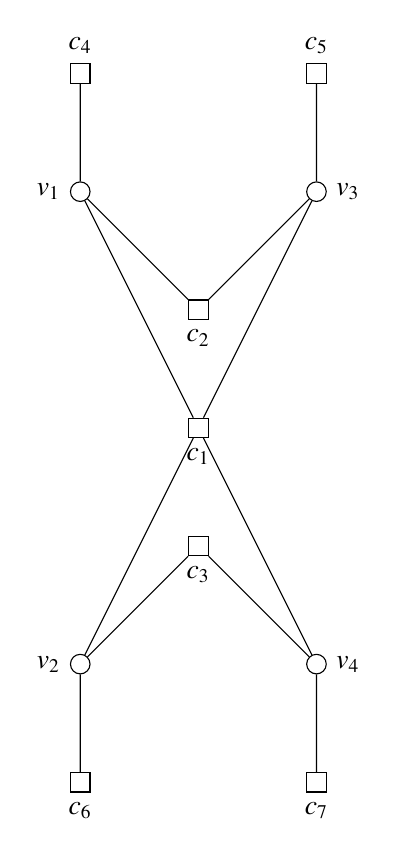
\begin{tikzpicture}[scale=0.5,square/.style={regular polygon,regular polygon sides=4},scale=3]

        \node[fill=white,draw=black,square,label=below:{$c_1$},scale=0.75] (c1) at (0,0) {};
        \node[fill=white,draw=black,square,label=below:{$c_2$},scale=0.75] (c2) at (0,1) {};
        \node[fill=white,draw=black,square,label=below:{$c_3$},scale=0.75] (c3) at (0,-1) {};
        \node[fill=white,draw=black,square,label=above:{$c_4$},scale=0.75] (c4) at (-1,3) {};
        \node[fill=white,draw=black,square,label=above:{$c_5$},scale=0.75] (c5) at (1,3) {};
        \node[fill=white,draw=black,square,label=below:{$c_6$},scale=0.75] (c6) at (-1,-3) {};
        \node[fill=white,draw=black,square,label=below:{$c_7$},scale=0.75] (c7) at (1,-3) {};

        \node[fill=white,draw=black,circle,label=left:{$v_1$},scale=0.75] (v1) at (-1,2) {};
        \node[fill=white,draw=black,circle,label=left:{$v_2$},scale=0.75] (v2) at (-1,-2) {};
        \node[fill=white,draw=black,circle,label=right:{$v_3$},scale=0.75] (v3) at (1,2) {};
        \node[fill=white,draw=black,circle,label=right:{$v_4$},scale=0.75] (v4) at (1,-2) {};

        \draw[thin] (c1) to (v1);
        \draw[thin] (c1) to (v2);
        \draw[thin] (c1) to (v3);
        \draw[thin] (c1) to (v4);
        \draw[thin] (c2) to (v1);
        \draw[thin] (c2) to (v3);
        \draw[thin] (c3) to (v2);
        \draw[thin] (c3) to (v4);
        \draw[thin] (c4) to (v1);
        \draw[thin] (c5) to (v3);
        \draw[thin] (c6) to (v2);
        \draw[thin] (c7) to (v4);
    \end{tikzpicture}
\end{center}

Corresponding matrix to the above graph:
$$\begin{bmatrix} 1 & 0 & 0 & 0 \\ 0 & 1 & 0 & 0 \\1 & 1 & 0 & 0 \\ 1 & 1 & 1 & 1 \\ 0 & 0 & 1 & 1 \\ 0 & 0 & 1 & 0 \\ 0 & 0 & 0 & 1
    \end{bmatrix}$$

Question: What relationship does a graph having a nonzero solution (i.e. all check nodes are satisfied with a set of variable node assignments such that not every variable node assignment is zero) to being an absorbing set?

\section*{11/15/2023}

Corrected definitions:
\begin{itemize}
    \item A trapping set is a set of variable nodes that does not eventually converge to a solution under a set iterative decoding rule.
    \item An absorbing set is a set of variable nodes that, assuming all variable nodes have an input of 1, under our iterative decoding rule, no variable node changes its value. (i.e. no 1 flips to a 0)
    \item In the classical $(u|s)$ setting, the above definition translates to for all $v \in D$, in $G_D$, $D_o(v) < D_e(v)$.
\end{itemize}

Prove this: Can we classify absorbing sets in $(u \mid s+k)$? Prove that this is when $D_o(v) \leq D_e(v) + k-1$. Yes, and this is a full characterization of absorbing sets under the $(u \mid s+k)$ update rule.

\begin{proof}
    Let the update rule be   $u\geq s+k$ and assume that for all $v\in S$ the inequality $D_o(v)\leq D_e(v)+k-1$ is true. Then initializing all variable nodes with $1$ then the for all variable nodes $u\leq s+k-1$ is true. Then changing to a strict inequality we have $u< s+k$ therefore no variable nodes would satisfy the update rule $u\geq s+k$.
\end{proof}



Fix an update rule. What is the minimal operation needed to break an absorbing set? What if we have to keep the code the same?

What if we change our update rule to be a fraction?

\section*{11/29/2023}





If we fix a class of codes, can we talk about breaking absorbing sets in a smart way that doesn't add new ones?


\section*{12/6/2023}

Collin's additions:

\begin{center}
    \begin{tikzpicture}[scale=0.5,square/.style={regular polygon,regular polygon sides=4},scale=3]

        \node[fill=white,draw=black,square,label=below:{$c_1$},scale=0.75] (c1) at (0,0) {};
        \node[fill=white,draw=black,square,label=below:{$c_2$},scale=0.75] (c2) at (0,2) {};
        \node[fill=white,draw=black,square,label=below:{$c_3$},scale=0.75] (c3) at (0,-2) {};
        \node[fill=white,draw=black,square,label=left:{$c_4$},scale=0.75] (c4) at (-1,0) {};
        \node[fill=white,draw=black,square,label=above:{$c_5$},scale=0.75] (c5) at (1,3) {};

        \node[fill=white,draw=black,square,label=below:{$c_6$},scale=0.75] (c7) at (1,-3) {};

        \node[fill=white,draw=black,square,label=below:{$c_7$},scale=0.75] (c8) at (2,-2) {};

        \node[fill=white,draw=black,square,label=right:{$c_8$},scale=0.75] (c9) at (1,0) {};



        \node[fill=white,draw=black,circle,label=left:{$v_1$},scale=0.75] (v1) at (-1,2) {};
        \node[fill=white,draw=black,circle,label=left:{$v_2$},scale=0.75] (v2) at (-1,-2) {};
        \node[fill=white,draw=black,circle,label=right:{$v_3$},scale=0.75] (v3) at (1,2) {};
        \node[fill=white,draw=black,circle,label=right:{$v_4$},scale=0.75] (v4) at (1,-2) {};

        \draw[thin] (c9) to (v3);
        \draw[thin] (c9) to (v4);

        \draw[thin] (v2) to (c4);
        \draw[thin] (c1) to (v1);

        \draw[thin] (c1) to (v4);
        \draw[thin] (c2) to (v1);
        \draw[thin] (c2) to (v3);
        \draw[thin] (c3) to (v2);
        \draw[thin] (c3) to (v4);
        \draw[thin] (c4) to (v1);
        \draw[thin] (c5) to (v3);
        \draw[thin] (v4) to (c8);

        \draw[thin] (c7) to (v4);
    \end{tikzpicture}
\end{center}


If we are only interested in determining whether something is in the set of words, then we can treat the graph as a Boolean function and use tools for finding equivalent functions. We can have the check nodes each be their own individual Boolean function that will yield zero if and only if the sum of the variable nodes is even. This can be done using the parity function; in this case, as they all have a degree of two, the parity function would simply be XOR. For example, looking at the check node $c_2$, we could create the Boolean function $c_2(a, b) = a\bar{b} + \bar{a}b$, where multiplication represents logical 'and,' addition is logical 'or,' and the overline denotes logical negation. Now, $c_2(1,0) = 1\bar{0} + \bar{0}0 = 1 \cdot 1 + 0 = 1$. So, if the output of the function is 1, then we know the number of 1's in the input was odd. If we repeat this process for the entire graph and add each individual check node in the parity function form, we get:

$$g(v_1, v_2, v_3, v_4) = v_1\bar{v_3} + \bar{v_1}v_3 + v_3 + v_3\bar{v_4} + \bar{v_3}v_4 + v_4 + v_4 + v_4\bar{v_2} + \bar{v_4}v_2 + v_1\bar{v_2} + \bar{v_1}v_2 + v_1\bar{v_4} + \bar{v_1}v_4$$

After simplifying, we find that this function is equal to:

$$g(v_1, v_2, v_3, v_4) = v_1 + v_2 + v_3 + v_4$$

A word is in the alphabet $A$ if and only if, after plugging it into the function, it is equal to 0. That is, $a \in A \iff g(a) = 0$. The tool I used to reduce the complexity of the function is called a Karnaugh map. This has no real use as you loose all information that matters to decoding the word as you do not have any information on satisfied and unsatisfied check nodes.


\end{document}